\documentclass[11pt]{article}

\usepackage[a4paper,margin=1in]{geometry}
\usepackage[T1]{fontenc}
\usepackage[utf8]{inputenc}
\usepackage{lmodern}
\usepackage{microtype}
\usepackage{xcolor}
\usepackage{amsmath,amssymb,amsthm,mathtools}
\usepackage{bm}
\usepackage{array,booktabs,longtable,multirow}
\usepackage{enumitem}
\usepackage{tikz}
\usetikzlibrary{arrows.meta,positioning,calc,fit}
\usepackage[most]{tcolorbox}
\usepackage{hyperref}
\usepackage{fancyhdr}
\usepackage{titlesec}
\usepackage{setspace}

\hypersetup{
  colorlinks=true,
  linkcolor=blue!50!black,
  urlcolor=blue!50!black,
  citecolor=blue!50!black,
  pdftitle={Coding Theory: Linear Codes and Distances - Lecture Notes}
}

\definecolor{accent}{RGB}{38,84,124}
\definecolor{softaccent}{RGB}{232,240,248}
\definecolor{softgray}{RGB}{245,246,248}
\definecolor{rulegray}{RGB}{214,219,224}

\titleformat{\section}{\large\bfseries\color{accent}}{\thesection.}{0.6em}{}
\titleformat{\subsection}{\normalsize\bfseries\color{accent}}{\thesubsection.}{0.6em}{}
\titleformat{\subsubsection}{\normalsize\bfseries}{\thesubsubsection.}{0.6em}{}

\setlength{\parindent}{0pt}
\setlength{\parskip}{0.55em}
\setstretch{1.08}
\setlength{\headheight}{14pt}

\pagestyle{fancy}
\fancyhf{}
\fancyhead[L]{\textit{Coding Theory Lecture Notes}}
\fancyhead[R]{\textit{Linear Codes and Distances}}
\fancyfoot[C]{\thepage}
\renewcommand{\headrulewidth}{0.4pt}
\renewcommand{\footrulewidth}{0pt}

\newtheorem{proposition}{Proposition}[section]
\newtheorem{theorem}[proposition]{Theorem}
\newtheorem{corollary}[proposition]{Corollary}
\theoremstyle{definition}
\newtheorem{definition}[proposition]{Definition}
\newtheorem{example}[proposition]{Example}
\newtheorem{exercise}[proposition]{Exercise}
\theoremstyle{remark}
\newtheorem*{remark}{Remark}

\newcommand{\F}{\mathbb{F}}
\newcommand{\code}{\mathcal{C}}
\newcommand{\dual}[1]{#1^{\perp}}
\newcommand{\wt}{\operatorname{wt}}
\newcommand{\dH}{d_{\mathrm H}}

\begin{document}
\pagenumbering{gobble}

\begin{titlepage}
\centering
\vspace*{2cm}

{\color{accent}\rule{0.82\textwidth}{1.2pt}}\par
\vspace{0.8cm}
{
  \Huge\bfseries Coding Theory\\[0.35em]
  \LARGE Linear Codes and Distances
}\par
\vspace{0.8cm}
{\color{accent}\rule{0.82\textwidth}{1.2pt}}\par
\vspace{1.2cm}

\begin{tcolorbox}[
  width=0.86\textwidth,
  colback=softaccent,
  colframe=accent!65,
  boxrule=0.8pt,
  arc=2mm,
  left=8pt,right=8pt,top=8pt,bottom=8pt
]
\large
These notes reorganize the slide deck into a continuous lecture-note format. The main goals are:
\begin{itemize}[leftmargin=1.4em,itemsep=0.35em,topsep=0.35em]
    \item to define the Hamming distance and the weight of a vector,
    \item to introduce the minimum distance of a linear code,
    \item to compute this distance for standard examples,
    \item to explain the link between minimum distance and erasure recovery,
    \item to characterize minimum distance using the parity-check matrix.
\end{itemize}
\end{tcolorbox}

\vfill
{\normalsize Prepared from the lecture slides \emph{Coding Theory: Linear Codes and Distances}.}

\end{titlepage}

pagenumbering{arabic}
\setcounter{page}{1}

\tableofcontents
\vspace{0.8em}

\begin{tcolorbox}[
  colback=softgray,
  colframe=rulegray,
  boxrule=0.6pt,
  arc=1.5mm,
  left=8pt,right=8pt,top=6pt,bottom=6pt,
  title=Notation,
  coltitle=black,
  fonttitle=\bfseries
]
Throughout, $\F_q$ denotes a finite field with $q$ elements. A linear $(n,k)$ code over $\F_q$ is a $k$-dimensional subspace of $\F_q^n$. We write vectors as row vectors unless explicitly transposed. For a code $\code$, the dual code is denoted by $\dual{\code}$.
\end{tcolorbox}

\section{The communication model and the matrix viewpoint}

We begin with the standard communication model already used in the previous lecture notes. A message
\[
x=(x_1,\dots,x_k)\in\F_q^k
\]
is encoded into a codeword
\[
c=(c_1,\dots,c_n)\in\F_q^n,\qquad n\ge k,
\]
which is then sent through a noisy channel.

\begin{center}
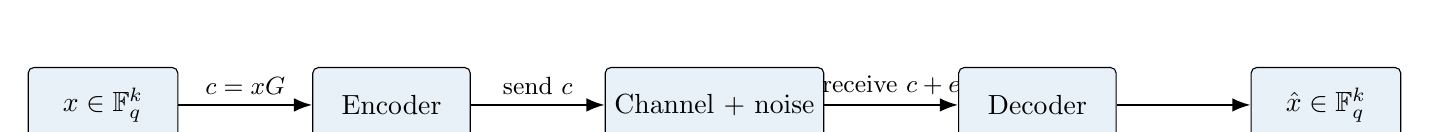
\begin{tikzpicture}[>=Latex, node distance=1.7cm]
  \node[draw, rounded corners=2pt, fill=softaccent, minimum width=1.9cm, minimum height=0.95cm] (data) {$x\in\F_q^k$};
  \node[draw, rounded corners=2pt, fill=softaccent, minimum width=2.0cm, minimum height=0.95cm, right=of data] (enc) {Encoder};
  \node[draw, rounded corners=2pt, fill=softaccent, minimum width=2.4cm, minimum height=0.95cm, right=of enc] (chan) {Channel + noise};
  \node[draw, rounded corners=2pt, fill=softaccent, minimum width=2.0cm, minimum height=0.95cm, right=of chan] (dec) {Decoder};
  \node[draw, rounded corners=2pt, fill=softaccent, minimum width=1.9cm, minimum height=0.95cm, right=of dec] (out) {$\hat x\in\F_q^k$};

  \draw[->, thick] (data) -- node[above, font=\small] {$c=xG$} (enc);
  \draw[->, thick] (enc) -- node[above, font=\small] {send $c$} (chan);
  \draw[->, thick] (chan) -- node[above, font=\small] {receive $c+e$} (dec);
  \draw[->, thick] (dec) -- (out);
\end{tikzpicture}
\end{center}

If $G$ is a generator matrix of an $(n,k)$ code $\code$, then
\[
\code=\{c=xG\mid x\in\F_q^k\}.
\]
If $H$ is a parity-check matrix, then the same code can be described as
\[
\code=\{v\in\F_q^n\mid Hv^T=0\}.
\]
The dual code is described by the analogous formulas
\[
\dual{\code}=\{c=xH\mid x\in\F_q^{n-k}\}
\qquad\text{and}\qquad
\dual{\code}=\{v\in\F_q^n\mid Gv^T=0\}.
\]
This lecture focuses on what the geometry of the code inside $\F_q^n$ tells us about error and erasure correction.

\section{Hamming distance and weight}

\subsection{Definition of Hamming distance}

\begin{definition}
For two vectors $x,y\in\F_q^n$, the \emph{Hamming distance} between $x$ and $y$ is the number of coordinates in which they differ. It is denoted by
\[
d(x,y)=\#\{i\in\{1,\dots,n\}: x_i\neq y_i\}.
\]
\end{definition}

So the Hamming distance simply counts how many coordinate positions have been changed.

\begin{proposition}
The Hamming distance is a genuine distance on $\F_q^n$. In other words, for all $x,y,z\in\F_q^n$:
\begin{align*}
d(x,y)&\ge 0,\\
d(x,y)&=0 \iff x=y,\\
d(x,y)&=d(y,x),\\
d(x,z)&\le d(x,y)+d(y,z).
\end{align*}
\end{proposition}

\begin{proof}
The first three properties follow directly from the definition.

For the triangle inequality, fix a coordinate $i$. If $x_i=z_i$, then this coordinate contributes nothing to $d(x,z)$. If $x_i\neq z_i$, then $y_i$ cannot agree with both $x_i$ and $z_i$ simultaneously. Thus at least one of the two comparisons $x_i\neq y_i$ or $y_i\neq z_i$ must hold. Summing over all coordinates gives
\[
d(x,z)\le d(x,y)+d(y,z).
\]
\end{proof}

\subsection{Weight of a vector}

\begin{definition}
For a vector $x=(x_1,\dots,x_n)\in\F_q^n$, the \emph{weight} of $x$ is the number of nonzero coordinates of $x$. It is denoted by
\[
\wt(x)=\#\{i\in\{1,\dots,n\}: x_i\neq 0\}.
\]
\end{definition}

\begin{example}
If $x=(1,0,1,0,0)$, then $\wt(x)=2$.
\end{example}

The weight and distance are related by a simple but fundamental identity.

\begin{proposition}
For all $x,y\in\F_q^n$,
\[
d(x,y)=\wt(x-y).
\]
\end{proposition}

\begin{proof}
The $i$-th coordinate of $x-y$ is zero exactly when $x_i=y_i$. Therefore the nonzero coordinates of $x-y$ are precisely the positions where $x$ and $y$ differ.
\end{proof}

\section{Minimum distance of a linear code}

For an arbitrary code, one defines the minimum distance by taking the minimum distance between distinct codewords. For linear codes, the previous proposition lets us simplify the definition.

\begin{definition}
Let $\code\subseteq\F_q^n$ be a nonzero linear code. Its \emph{minimum Hamming distance} is
\[
\dH(\code)=\min\{\wt(c): c\in\code,\ c\neq 0\}.
\]
If $\dH(\code)=d$, one sometimes writes that $\code$ is an $(n,k,d)$ code.
\end{definition}

\begin{remark}
This definition works because $\code$ is linear. Indeed,
\[
\min_{x\neq y\in\code} d(x,y)=\min_{x\neq y\in\code}\wt(x-y),
\]
and since $x-y\in\code$, the problem reduces to the minimum weight of a nonzero codeword.
\end{remark}

\section{Examples of minimum distance}

\subsection{The repetition code}

Consider the $(n,1)$ repetition code over $\F_q$, defined by
\[
(x_1)\longmapsto (x_1,\dots,x_1).
\]
Over $\F_2$, the only nonzero codeword is $(1,\dots,1)$, whose weight is $n$. More generally, over any $\F_q$, every nonzero codeword has all $n$ coordinates nonzero.

\begin{proposition}
The $(n,1)$ repetition code has minimum distance
\[
\dH(\code)=n.
\]
\end{proposition}

\begin{proof}
Every nonzero codeword has the form $(a,\dots,a)$ with $a\neq 0$. Hence all $n$ coordinates are nonzero, so its weight is $n$. Therefore the minimum nonzero weight is $n$.
\end{proof}

\subsection{The single parity-check code}

Consider the $(n,n-1)$ single parity-check code over $\F_q$ with encoding
\[
(x_1,\dots,x_{n-1})\longmapsto \left(x_1,\dots,x_{n-1},\sum_{i=1}^{n-1}x_i\right).
\]

\begin{proposition}
The single parity-check code has minimum distance
\[
\dH(\code)=2.
\]
\end{proposition}

\begin{proof}
The codeword
\[
(1,0,\dots,0,1)
\]
has weight $2$, so $\dH(\code)\le 2$.

A codeword of weight $1$ cannot occur. If exactly one information coordinate is nonzero, then the parity symbol is also nonzero, so the weight is at least $2$. If at least two information coordinates are nonzero, then again the weight is at least $2$. Hence no nonzero codeword has weight $1$, and therefore $\dH(\code)=2$.
\end{proof}

\subsection{\texorpdfstring{The $(7,4)$ Hamming code over $\F_2$}{The (7,4) Hamming code over F2}}

The slides use the generator matrix
\[
G=
\begin{bmatrix}
1&0&0&0&0&1&1\\
0&1&0&0&1&0&1\\
0&0&1&0&1&1&0\\
0&0&0&1&1&1&1
\end{bmatrix}.
\]
Thus the encoding map is
\[
x\longmapsto (x_1,x_2,x_3,x_4,\ x_2+x_3+x_4,\ x_1+x_3+x_4,\ x_1+x_2+x_4).
\]

\begin{proposition}
The $(7,4)$ Hamming code above has minimum distance
\[
\dH(\code)=3.
\]
\end{proposition}

\begin{proof}
Take $x=(1,0,0,0)$. Then
\[
xG=(1,0,0,0,0,1,1),
\]
which has weight $3$. So $\dH(\code)\le 3$.

Now we show that no nonzero codeword has weight $1$ or $2$. A codeword of weight $1$ is impossible because the parity coordinates are linked to the information coordinates by linear relations. If only one information bit is nonzero, the codeword produced by the matrix $G$ has weight $3$, as just seen. If two information bits are nonzero, then the corresponding parities cannot all vanish simultaneously, because the information bits appear in different parity positions. Hence every nonzero codeword has weight at least $3$. Therefore $\dH(\code)=3$.
\end{proof}

\subsection{The tetracode}

The $(4,2)$ tetracode over $\F_3$ is generated by
\[
G=
\begin{bmatrix}
1&0&1&1\\
0&1&1&-1
\end{bmatrix},
\]
so its codewords are of the form
\[
(x_1,x_2,x_1+x_2,x_1-x_2).
\]

\begin{proposition}
The tetracode has minimum distance
\[
\dH(\code)=3.
\]
\end{proposition}

\begin{proof}
If we take $x=(1,0)$, then the corresponding codeword is
\[
(1,0,1,1),
\]
which has weight $3$. So $\dH(\code)\le 3$.

To obtain a codeword of smaller weight, we would need at least two of the four coordinates to be zero. If both parity coordinates vanished, then we would have
\[
x_1+x_2=0,\qquad x_1-x_2=0.
\]
Adding and subtracting these equations in $\F_3$ gives $x_1=x_2=0$, so the codeword would be zero. Hence no nonzero codeword has weight $1$ or $2$. Therefore $\dH(\code)=3$.
\end{proof}

\subsection{Summary table}

\begin{center}
\renewcommand{\arraystretch}{1.2}
\begin{tabular}{@{}cccccc@{}}
\toprule
$n$ & $k$ & field & name & generator form & $\dH$ \\
\midrule
$n$ & $1$ & $\F_q$ & repetition & $(x_1)\mapsto(x_1,\dots,x_1)$ & $n$ \\
$n$ & $n-1$ & $\F_q$ & single parity-check & $(x_1,\dots,x_{n-1},\sum x_i)$ & $2$ \\
$7$ & $4$ & $\F_2$ & Hamming & matrix above & $3$ \\
$4$ & $2$ & $\F_3$ & tetracode & $(x_1,x_2,x_1+x_2,x_1-x_2)$ & $3$ \\
\bottomrule
\end{tabular}
\end{center}

\section{Minimum distance and erasure recovery}

The slides emphasize the erasure channel rather than the error channel. In an erasure channel, some positions are marked as unknown, often with the symbol $*$, but we know \emph{which} coordinates were lost.

\begin{theorem}
Let $\code$ be an $(n,k)$ linear code over $\F_q$ with minimum distance $\dH(\code)=d$. Then $\code$ can recover from up to $d-1$ erasures.
\end{theorem}

\begin{proof}
Take two distinct codewords $c,c'\in\code$. Since the minimum distance is $d$, they differ in at least $d$ coordinates. Therefore, after erasing at most $d-1$ coordinates, there is still at least one remaining coordinate in which $c$ and $c'$ differ. So the partially received word cannot be compatible with both codewords.

Hence a received word with at most $d-1$ erasures determines at most one codeword, which means the original codeword can be recovered uniquely.
\end{proof}

\begin{remark}
The theorem is sharp. If $d$ coordinates are erased, then two different codewords that differ exactly in those $d$ positions become indistinguishable.
\end{remark}

\subsection{\texorpdfstring{Example: the $(4,3,2)$ single parity-check code over $\F_2$}{Example: the (4,3,2) single parity-check code over F2}}

Its codewords are
\[
\begin{aligned}
&(0,0,0,0),\ (1,0,0,1),\ (0,1,0,1),\ (1,1,0,0),\\
&(0,0,1,1),\ (1,0,1,0),\ (0,1,1,0),\ (1,1,1,1).
\end{aligned}
\]
Since $\dH(\code)=2$, this code recovers from exactly one erasure.

For example, if we receive
\[
(0,*,1,0),
\]
then the unique compatible codeword is
\[
(0,1,1,0).
\]
But if we receive
\[
(0,*,1,*),
\]
then both
\[
(0,1,1,0)\qquad\text{and}\qquad (0,0,1,1)
\]
are compatible, so recovery is impossible.

\subsection{\texorpdfstring{Example: the tetracode over $\F_3$}{Example: the tetracode over F3}}

The tetracode consists of the nine codewords
\[
\begin{aligned}
&(0,0,0,0),\ (0,1,1,2),\ (0,2,2,1),\ (1,0,1,1),\ (1,1,2,0),\\
&(1,2,0,2),\ (2,0,2,2),\ (2,1,0,1),\ (2,2,1,0).
\end{aligned}
\]
Since $\dH(\code)=3$, the code can recover from up to two erasures.

If we receive
\[
(0,*,*,0),
\]
then the only compatible codeword is
\[
(0,0,0,0).
\]
But if we receive
\[
(*,*,1,*),
\]
then several codewords are compatible, namely
\[
(0,1,1,2),\qquad (1,0,1,1),\qquad (2,2,1,0).
\]
This is consistent with the theorem: three erasures may exceed the recovery capability.

\section{Parity-check matrices and minimum distance}

A second method for computing the minimum distance uses the parity-check matrix.

\subsection{From a codeword to a linear dependence}

Let $H=[h_1\ \cdots\ h_n]$ be the parity-check matrix of a linear code $\code$, where $h_i$ denotes the $i$-th column of $H$. If
\[
c=(c_1,\dots,c_n)\in\code,
\]
then $Hc^T=0$, which means
\[
c_1h_1+c_2h_2+\cdots+c_nh_n=0.
\]
Thus the columns of $H$ corresponding to the nonzero coordinates of $c$ are linearly dependent.

\begin{proposition}
If $c\in\code$ is a nonzero codeword, then the columns of $H$ indexed by the support of $c$ form a linearly dependent set.
\end{proposition}

\begin{proof}
Since $c\in\code$, we have $Hc^T=0$. Writing $H$ by columns gives
\[
Hc^T=c_1h_1+\cdots+c_nh_n=0.
\]
Only the nonzero coefficients $c_i$ matter, so the corresponding columns are linearly dependent.
\end{proof}

\subsection{From a linear dependence to a codeword}

Conversely, suppose there is a linear relation
\[
v_1h_1+v_2h_2+\cdots+v_nh_n=0
\]
with exactly $w$ nonzero coefficients $v_i$. If we set
\[
v=(v_1,\dots,v_n),
\]
then $Hv^T=0$, so $v\in\code$, and by construction $\wt(v)=w$.

\begin{proposition}
If a set of $w$ columns of $H$ is linearly dependent, then $\code$ contains a codeword of weight $w$ whose nonzero coordinates correspond to those columns.
\end{proposition}

\begin{proof}
A linear dependence among those columns gives coefficients $v_i$, not all zero, such that
\[
\sum_{i=1}^n v_i h_i=0.
\]
Equivalently, $Hv^T=0$, so $v\in\code$. The nonzero coefficients occur exactly at the chosen $w$ columns, hence $\wt(v)=w$.
\end{proof}

Combining the two directions yields the main criterion.

\begin{theorem}
Let $\code$ be a linear code with parity-check matrix $H$. Then $\dH(\code)=d$ if and only if:
\begin{itemize}[leftmargin=1.4em]
    \item some set of $d$ columns of $H$ is linearly dependent, and
    \item every set of $d-1$ columns of $H$ is linearly independent.
\end{itemize}
\end{theorem}

\begin{proof}
If $\dH(\code)=d$, then there exists a codeword of weight $d$, so the corresponding $d$ columns of $H$ are linearly dependent. If there were a dependent set of fewer than $d$ columns, the previous proposition would produce a codeword of weight less than $d$, contradiction.

Conversely, if the smallest number of dependent columns is $d$, then the second proposition gives a codeword of weight $d$, and no codeword of smaller weight can exist. Hence $\dH(\code)=d$.
\end{proof}

\section{Examples via parity-check matrices}

\subsection{The repetition code}

For the repetition code, a parity-check matrix in systematic form is
\[
H=
\begin{bmatrix}
-1 & 1 & 0 & \cdots & 0\\
-1 & 0 & 1 & \cdots & 0\\
\vdots & \vdots & \vdots & \ddots & \vdots\\
-1 & 0 & 0 & \cdots & 1
\end{bmatrix}.
\]
The first column is the negative of the sum of the remaining $n-1$ columns, so all $n$ columns are linearly dependent. On the other hand, any $n-1$ columns are linearly independent. Therefore the parity-check characterization gives
\[
\dH(\code)=n.
\]

\subsection{The $(7,4)$ Hamming code}

The parity-check matrix used in the slides is
\[
H=
\begin{bmatrix}
0&1&1&1&1&0&0\\
1&0&1&1&0&1&0\\
1&1&0&1&0&0&1
\end{bmatrix}.
\]
The columns $4,5,6,7$ are linearly dependent. In fact, the columns $1,6,7$ are already linearly dependent. But any two columns are linearly independent. Therefore the smallest size of a dependent set is $3$, so
\[
\dH(\code)=3.
\]

\section{Final summary}

\begin{tcolorbox}[
  colback=softaccent,
  colframe=accent!65,
  boxrule=0.8pt,
  arc=2mm,
  title=Key facts,
  fonttitle=\bfseries,
  coltitle=black
]
\begin{enumerate}[leftmargin=1.5em,itemsep=0.35em]
    \item For vectors in $\F_q^n$, the Hamming distance counts the number of coordinates in which they differ.
    \item The weight of a vector is the number of its nonzero coordinates, and $d(x,y)=\wt(x-y)$.
    \item For a linear code $\code$, the minimum distance is the minimum weight of a nonzero codeword.
    \item A code with minimum distance $d$ can recover from up to $d-1$ erasures.
    \item If $H$ is a parity-check matrix of $\code$, then $\dH(\code)=d$ exactly when $H$ has a dependent set of $d$ columns but no dependent set of $d-1$ columns.
\end{enumerate}
\end{tcolorbox}

\begin{center}
\renewcommand{\arraystretch}{1.18}
\begin{tabular}{@{}lccc@{}}
\toprule
Code & Parameters & Minimum distance & Erasure recovery \\
\midrule
Repetition code & $(n,1,n)$ & $n$ & $n-1$ erasures \\
Single parity-check code & $(n,n-1,2)$ & $2$ & $1$ erasure \\
Hamming code & $(7,4,3)$ & $3$ & $2$ erasures \\
Tetracode & $(4,2,3)$ over $\F_3$ & $3$ & $2$ erasures \\
\bottomrule
\end{tabular}
\end{center}

\end{document}
